\subsection{Elipse}

\begin{figure}[h]
\centering
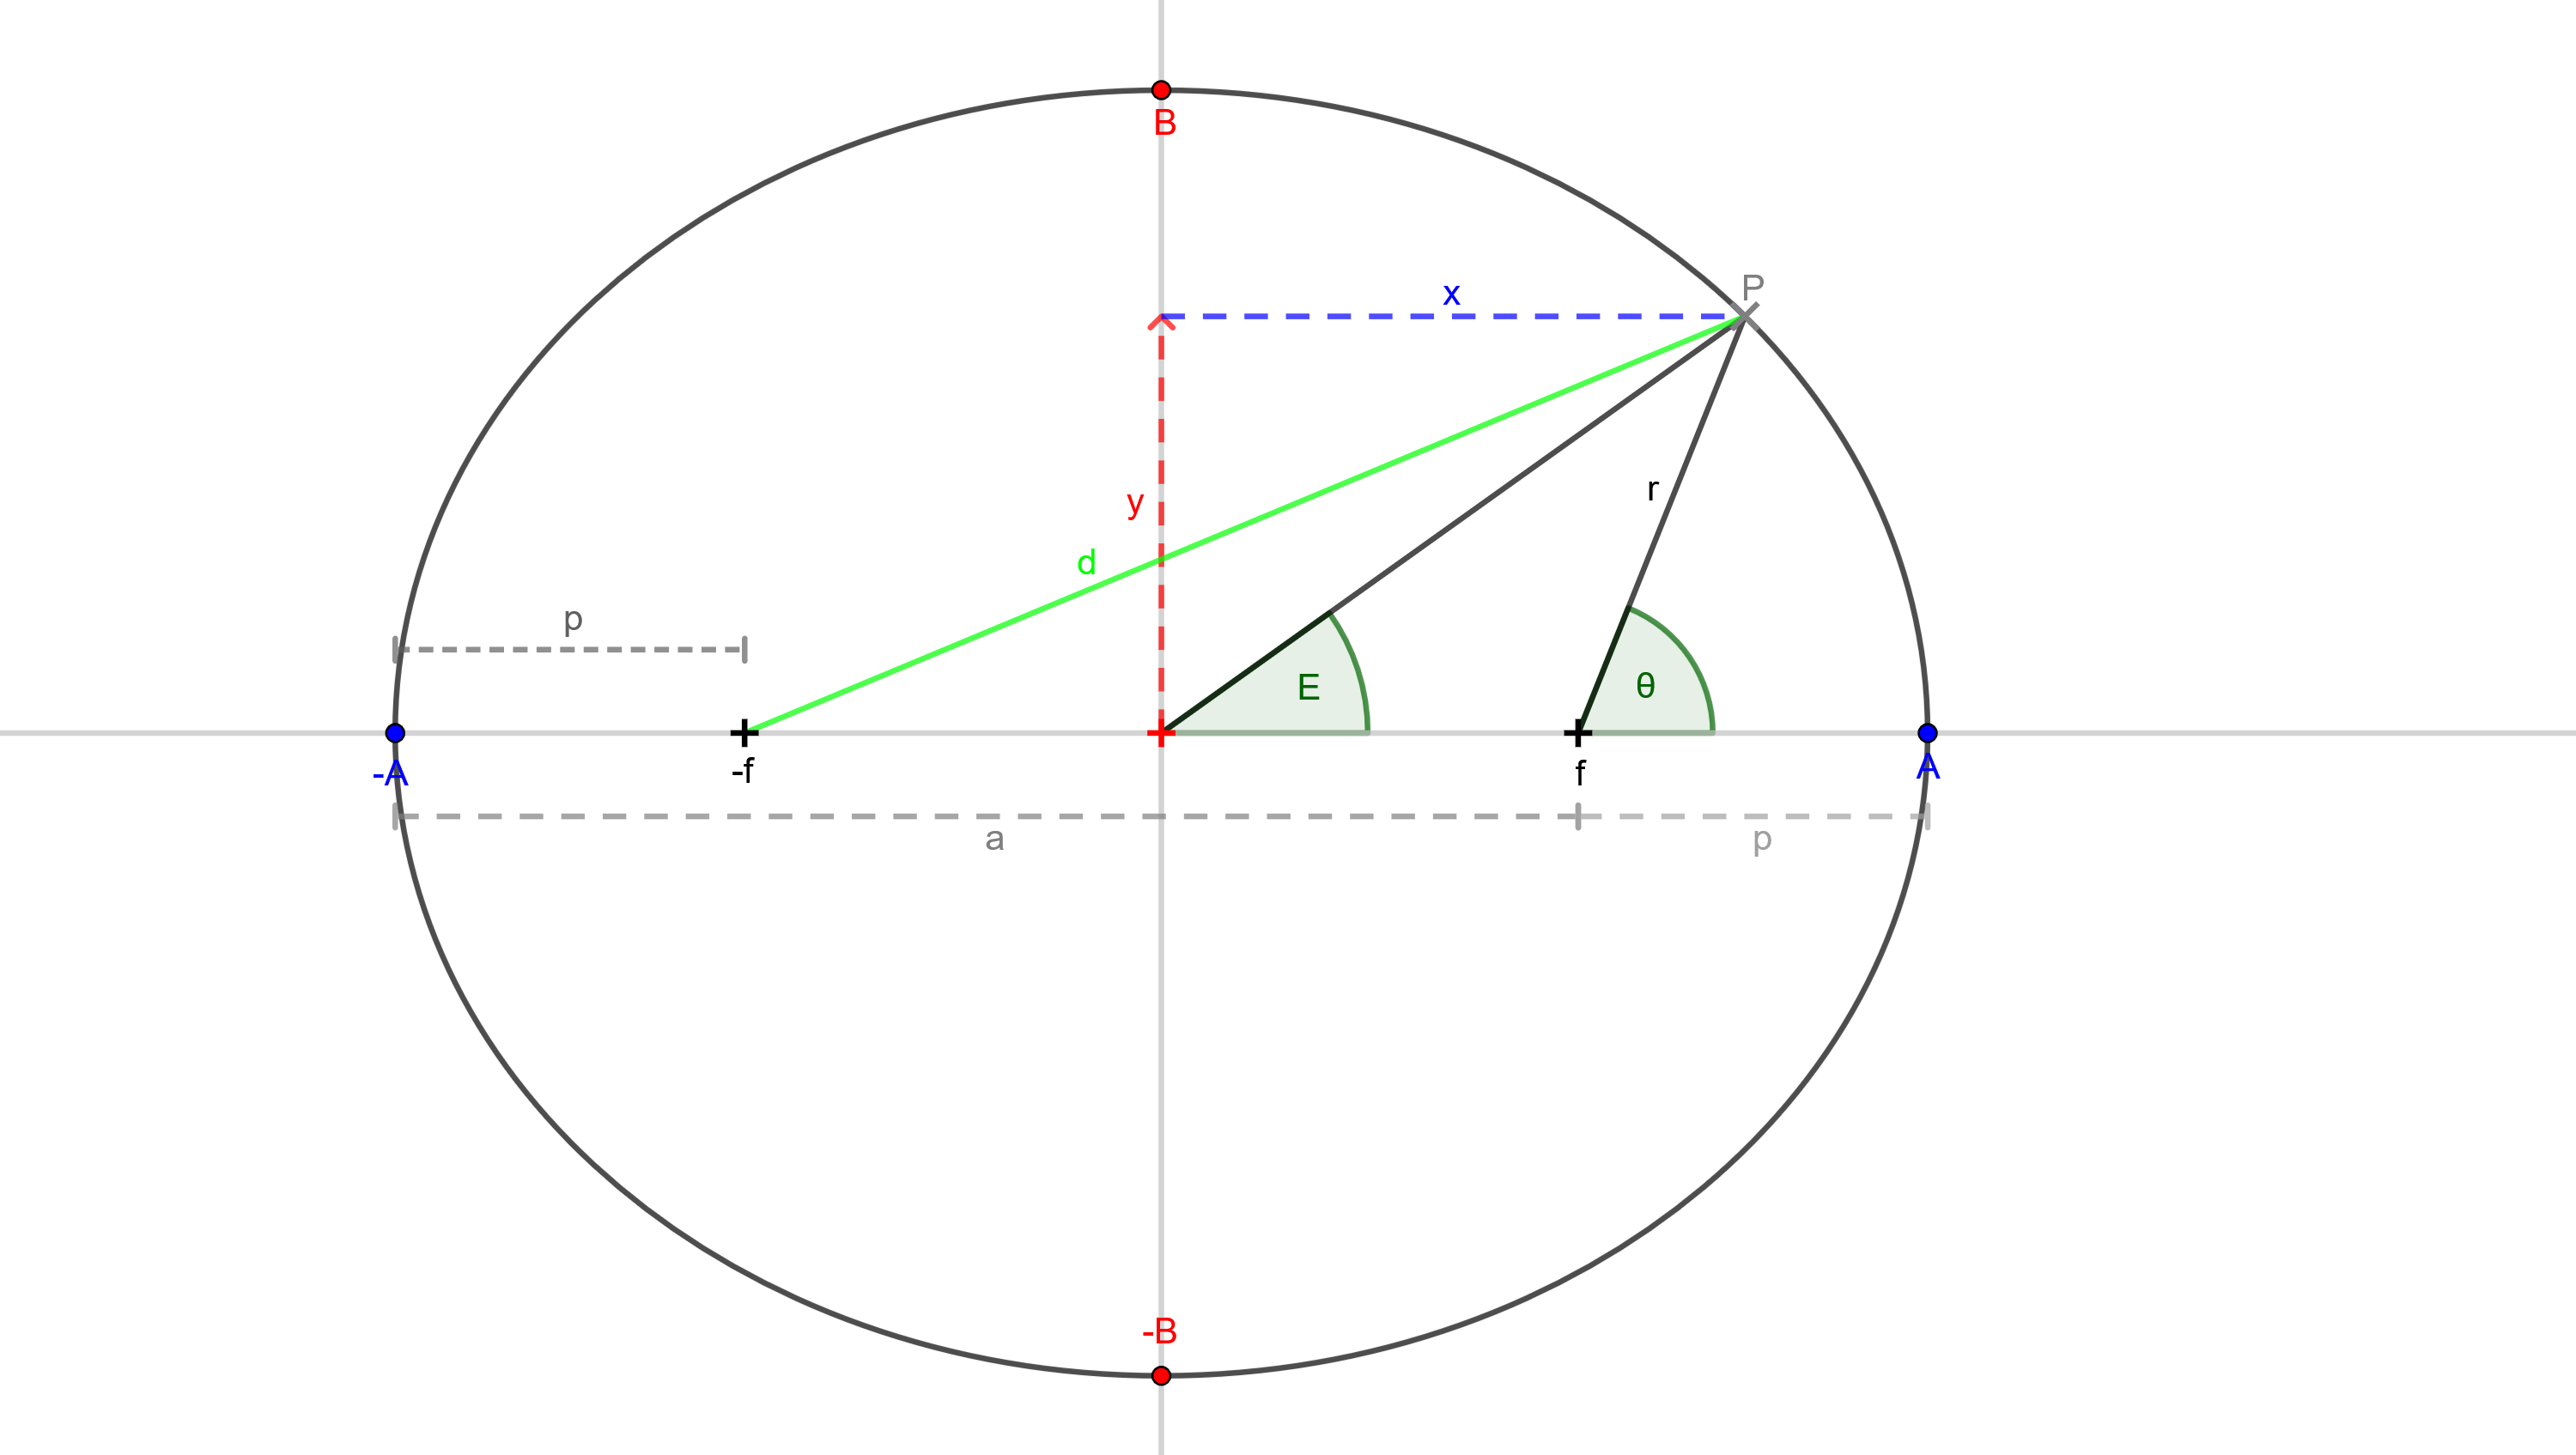
\includegraphics[width=0.8\textwidth]{./img/elipse.png} 
\caption{An Elipse with important values shown} \label{fig:GeometryElipse}
\end{figure}

In the above diagram a point $P$ on the ellipse forms an angle $E$ with the origin and the $x$ axis. Also the angle $\theta$ is formed at the ellipse's focus between the point on the ellipse and the axis.

We also define the distances $a$ and $p$ as the apoapsis and periapsis distances respectively.

The semi major axis has been labeled as $A$, so that the total width of the ellipse is $2A$. Also shown on the diagram is the semi minor axis $B$, so the total height of the ellipse is $2B$.

For this text we will take the elliptical eccentricity to be defined as the ratio of the focus and the semi major axis.
\begin{equation}
e = \frac{f}{A}
\end{equation}
\subsubsection{The Apses}
Before we get any further, we will look at the apses. From figure \ref{fig:GeometryElipse} we can see that

\begin{equation}
p = A - f = A - eA = A(1-e)
\end{equation}

and that
\begin{equation}
a  = A + f = A + eA = A(1+e)
\end{equation}

also

\begin{align}
a+p &= A -f + A +f = 2A \\
a-p &= A + f - A + f = 2f
\end{align}

which can give us the eccentricity as defined by the apses
\begin{equation}
e=\frac{f}{A}=\frac{2f}{2A}=\frac{a-p}{a+p}
\end{equation}

\subsubsection{Sum of distances from foci and $P$}

One property of an ellipse is that the sum of the distances from any point on the ellipse and the foci is a constant. This fact allows you to draw an ellipse using two pins and a piece of string. We will use this fact and look at two special cases, before looking at the general case and deriving the equation for an ellipse. Before we do we will define what the sum is here.

\begin{equation}
S=d+r
\end{equation}

\paragraph{Special Case 1: Point on the $x$ axis}

When the point is at $(A,0)$. The distance $d$ is $f+A$ and the distance $r$ is $A-f$ from the diagram above. So our sum becomes

\begin{equation}
S = d + r = f+A + A-f = 2A
\end{equation}

\paragraph{Special Case 2: Point on the $y$ axis}



\subsection{Solving equtaions of motion}

Firstly we let $r=\frac{1}{u}$, so that

\begin{align}
\frac{dr}{dt} &= \frac{du^{-1}}{dt}\nonumber \\
&= \frac{du^{-1}}{du}\frac{du}{dt}\nonumber \\
&= -\frac{1}{u^2}\frac{du}{dt}\nonumber \\
&= -r^2\frac{du}{dt}
\end{align}

next we introduce an $\omega$ by chain rule

\begin{align}
\frac{dr}{dt}
&= -r^2\frac{du}{dt}\nonumber \\
\frac{dr}{dt} &= -r^2\frac{du}{d\theta}\frac{d\theta}{dt} \nonumber \\
&= -r^2\omega\frac{du}{d\theta} \nonumber
\end{align}

And using the magnitude of angular momentum\footnote{equation \ref{eq:AngularMomentumScalar}} $l=mr^2\omega$ or rearranging $\omega = \frac{l}{mr^2}$

\begin{align}
\frac{dr}{dt}&= -r^2\omega\frac{du}{d\theta} \nonumber \\
\frac{dr}{dt}&= -r^2\frac{l}{mr^2}\frac{du}{d\theta} \nonumber \\
\frac{dr}{dt}&= -\frac{l}{m}\frac{du}{d\theta} \nonumber \\
\frac{dr}{dt}&= -\frac{l}{m}\frac{du}{d\theta}
\end{align}

Differentiating again with respect to time gives

\begin{align}
\frac{dr^2}{dt^2}&= -\frac{l}{m}\frac{d}{dt}\frac{du}{d\theta} \nonumber \\
&= -\frac{l}{m}\frac{d\theta}{dt}\frac{d}{d\theta}\frac{du}{d\theta}\nonumber \\
&= -\frac{l}{m}\omega\frac{d^2u}{d\theta^2}
\end{align}

We can substitute the magnitude of angular momentum\footnote{equation \ref{eq:AngularMomentumScalar}} $l=mr^2\omega$ again to get

\begin{align}
\frac{dr^2}{dt^2}&= -\frac{l}{m}\omega\frac{d^2u}{d\theta^2} \nonumber \\
&= -\frac{mr^2\omega}{m}\omega\frac{d^2u}{d\theta^2} \nonumber \\
&= -r^2\omega^2\frac{d^2u}{d\theta^2}
\end{align}

We can now substitute this into the radial part of the acceleration\footnote{equation \ref{eq:radialAcceleration}}

\begin{align}
-\frac{GM}{r^2}&= \frac{ d^2 r}{d t^2} -r \omega^2  \nonumber \\
&=-r^2\omega^2\frac{d^2u}{d\theta^2} -r\omega^2 \nonumber \\
&=-r^2\omega^2\left[\frac{d^2u}{d\theta^2}+\frac{1}{r}\right] \nonumber \\
GM&=r^4\omega^2\left[\frac{d^2u}{d\theta^2}+\frac{1}{r}\right]
\end{align}

Next we recall that $u=\frac{1}{r}$ and that $\frac{l}{m}=r^2\omega$ and substitute these in

\begin{align}
GM&=\left(\frac{l}{m}\right)^2\left[\frac{d^2u}{d\theta^2}+u\right] \nonumber\\
\frac{d^2u}{d\theta^2}+u &=\frac{GMm^2}{l^2}
\end{align}

To simplify this equation we will use $\alpha=\frac{GMm^2}{l^2}$

\subsubsection{Solution}

The direct solution to
\begin{equation}
\frac{d^2u}{d\theta^2}+u =\alpha
\end{equation}

is $u=\alpha$

However because there is also a function that results in zero, we must include that

\begin{align}
\frac{d^2u}{d\theta^2}+u &=0 \nonumber \\
\frac{d^2u}{d\theta^2} &=-u
\end{align}

we can take the solution that $u=c\cos\theta$ which gives the general overall solution of

\begin{equation}
u(\theta)=\alpha + c \cos \theta
\end{equation}

We can pick an initial condition when $\theta=0$ the body is at periapsis or $r=p=A(1-e)$ which gives $u=\frac{1}{A(1-e)}$ (see the ellipse notes for $p=A(1-e)$)


\begin{align}
\frac{1}{A(1-e)}&=\alpha+c \nonumber \\
\alpha&=\frac{1}{A(1-e)} - c
\end{align}


we could similarly hae picked the condition that when $\theta=\pi$ the body is at apoapsis or $r=a=A(1+e)$ which gives $u=\frac{1}{A(1+e)}$ (see ellipse notes for $a=A(1+e)$)


\begin{align}
\frac{1}{A(1+e)}&=\alpha-c \nonumber \\
\alpha&=\frac{1}{A(1+e)} + c
\end{align}

we can equate our two initial conditions to get $c$ in terms of just $a$ and $p$

\begin{align}
\alpha=\frac{1}{A(1-e)}-c&=\frac{1}{A(1+e)} + c \nonumber \\
\frac{1}{A(1-e)}-\frac{1}{A(1+e)}&=2c \nonumber \\
\frac{A(1+e)-A(1-e)}{A^2(1+e)(1-e)}&=2c \nonumber \\
\frac{A+eA-A+eA}{A^2(1-e^2)}&=2c \nonumber \\
\frac{2eA}{A^2(1-e^2)}&=2c \nonumber \\
\frac{e}{A(1-e^2)}&=c
\end{align}

Now that we have $c$ we can use this to determine $\alpha$ in terms of $A$ and $e$

\begin{align}
\alpha&=\frac{1}{A(1+e)} + c \nonumber \\
&=\frac{1}{A(1+e)} + \frac{e}{A(1-e)^2}\nonumber \\
&=\frac{(1-e)}{A(1+e)(1-e)} + \frac{e}{A(1-e)^2}\nonumber \\
&=\frac{1-e+e}{A(1-e^2)} \nonumber \\
&=\frac{1}{A(1-e^2)} \nonumber
\end{align}

So feeding all this back in we have

\begin{align}
u(\theta)&=\alpha + c \cos \theta \nonumber \\
&=\frac{1}{A(1-e^2)} + \frac{e}{A(1-e^2)} \cos \theta \nonumber \\
&=\frac{1+e\cos\theta}{A(1-e^2)}
\end{align}

Now we have a simple form for $u$ we can recall that we chose $u=\frac{1}{r}$, so

\begin{equation}
r=\frac{1+e\cos\theta}{A(1-e^2)}
\end{equation}

which is the equation for a ellipse we saw from the ellipse notes.

We also get the interesting result here that

\begin{align}
\alpha = \frac{GMm^2}{l^2}&=\frac{1}{A(1-e^2)} \nonumber \\
A(1-e^2)&=\frac{l^2}{GMm^2}
\end{align}
